\documentclass[11pt,a4paper]{article}
\usepackage[utf8]{inputenc}
\usepackage[T1]{fontenc}
\usepackage{lmodern}
\usepackage[a4paper,margin=2.1cm,headheight=14pt]{geometry}
\usepackage{xcolor,graphicx,booktabs,longtable,tabularx,array,enumitem,fancyhdr,titlesec,hyperref,makecell}
\usepackage[most]{tcolorbox}
\usepackage{pgfgantt}
\definecolor{navy}{HTML}{1B3A5C}
\definecolor{gold}{HTML}{C9A227}
\definecolor{light}{HTML}{EEF2F7}
\hypersetup{colorlinks=true,linkcolor=navy,urlcolor=navy}
\titleformat{\section}{\Large\bfseries\color{navy}}{\thesection}{0.6em}{}[{\color{gold}\titlerule[1.2pt]}]
\titleformat{\subsection}{\large\bfseries\color{navy}}{\thesubsection}{0.5em}{}
\titleformat{\subsubsection}{\normalsize\bfseries\color{navy}}{\thesubsubsection}{0.5em}{}
\titlespacing*{\section}{0pt}{10pt}{6pt}
\titlespacing*{\subsection}{0pt}{8pt}{4pt}
\setlist{itemsep=1pt,topsep=3pt}
\renewcommand{\arraystretch}{1.18}
\pagestyle{fancy}\fancyhf{}
\fancyhead[L]{\small\color{navy} MaintiDoc -- Livrable 1 : cadrage, corpus et architecture}
\fancyhead[R]{\small\color{navy} ELMECHRAFI-GHZAOUNI}
\fancyfoot[C]{\small \thepage}
\renewcommand{\headrulewidth}{0.4pt}
\newtcolorbox{idee}[1][]{colback=light,colframe=navy,fonttitle=\bfseries,title=#1,boxrule=0.6pt,arc=2pt,left=5pt,right=5pt,top=3pt,bottom=3pt}
\newtcolorbox{alerte}[1][]{colback=gold!12,colframe=gold!85!black,fonttitle=\bfseries\color{black},title=#1,boxrule=0.6pt,arc=2pt,left=5pt,right=5pt,top=3pt,bottom=3pt}
\newcolumntype{L}[1]{>{\raggedright\arraybackslash}p{#1}}
\setlength{\parskip}{3pt}

\renewcommand{\contentsname}{Sommaire}\renewcommand{\figurename}{Figure}
\begin{document}
% ------------------------------------------------------------------ PAGE DE GARDE
\begin{titlepage}
\begin{tcolorbox}[colback=navy,colframe=navy,arc=0pt,left=14pt,top=16pt,bottom=16pt]
\color{white}{\large EMSI -- École Marocaine des Sciences de l'Ingénieur}\\[2pt]
{\small Module IA générative multimodale -- 2026}
\end{tcolorbox}
\vspace{3cm}
{\color{navy}\Huge\bfseries MaintiDoc}\\[6pt]
{\Large Assistant documentaire multimodal et agentique pour la maintenance}\\[4pt]
{\color{gold}\rule{\linewidth}{2pt}}\\[8pt]
{\LARGE\bfseries Livrable 1 sur 6 : cadrage, corpus et architecture}\\[4pt]
{\large Semaine 1}
\vfill
\begin{tabular}{@{}ll}
\textbf{Équipe} & ELMECHRAFI-GHZAOUNI \\
\textbf{Membres} & Salah ELMECHRAFI, Adam GHZAOUNI \\
\textbf{Enseignante} & Prof. Mariam CHERRABI \\
\textbf{Familles d'équipements} & pompes centrifuges et compresseurs \\
\textbf{Date} & novembre 2026 \\
\end{tabular}
\vspace{1.5cm}
\end{titlepage}

\tableofcontents
\vspace{6pt}
\begin{idee}[Le livrable en un coup d'œil]
\begin{itemize}
\item \textbf{Corpus} : 44 documents synthétiques (110 pages), 2 familles, 3 PDF scannés, 6 photographies, 25 documents avec figures, schémas ou photos, 2 documents en anglais, 2 paires contradictoires, 2 documents piégés, 4 cas ambigus.
\item \textbf{Cohérence vérifiée par script} : codes d'alarme, équipements, références croisées, numéros d'intervention et inventaire contrôlés automatiquement.
\item \textbf{Architecture} : 7 blocs fonctionnels et 5 points de contrôle (droits, filtrage, citations, validation humaine, contrôle serveur MCP).
\item \textbf{Risques} : 12 risques cotés, avec une mesure et un responsable pour chacun.
\end{itemize}
\end{idee}
\newpage

% ================================================================== 2.1
\section{Cadrage du projet}
\subsection{Contexte et utilisateurs}
Dans un atelier, la bonne information existe presque toujours, mais elle est éparpillée entre un manuel de 10 pages, une procédure révisée l'an dernier, un schéma affiché dans le local et l'historique des interventions. MaintiDoc rassemble ces sources pour répondre à une question posée avec une photo, en citant la page et la figure qui justifient chaque affirmation. Il prépare un ticket de maintenance, mais seul un humain peut le valider.

\begin{center}
\begin{tabularx}{\linewidth}{L{3.1cm}X X}
\toprule
\textbf{Profil} & \textbf{Besoins} & \textbf{Droits dans le prototype}\\\midrule
Technicien pompes (\texttt{tech\_pompe\_01}, \texttt{tech\_pompe\_02}) & Interpréter un voyant, retrouver une procédure et ses valeurs (couple, huile), consulter l'historique d'une pompe & Documents des pompes ; peut préparer un ticket et l'approuver pour ses équipements\\
Technicien compresseurs (\texttt{tech\_comp\_01}) & Mêmes besoins pour les compresseurs à vis et à piston & Documents des compresseurs uniquement\\
Responsable maintenance (\texttt{resp\_maint\_01}) & Vue d'ensemble, plans préventifs, arbitrage entre documents contradictoires & Tout le corpus, y compris les plans préventifs et notes de service\\
\bottomrule
\end{tabularx}
\end{center}

\subsubsection*{Cas d'usage}
\begin{enumerate}[label=\textbf{CU\arabic*}]
\item \textbf{Voyant sur photo} : un technicien photographie le panneau de POMPE-A-01 (voyant orange) et demande sa signification. Sans code visible, l'assistant liste les causes possibles (A03, A04, A06, A07, A09) en citant le tableau 6.1 du manuel (page 6), puis demande le code affiché par la supervision.
\item \textbf{Code affiché} : photo de l'écran de COMP-V-01 affichant C06. L'assistant identifie un séparateur d'huile colmaté (manuel CV-37, tableau 6.1, p.6) et renvoie à la procédure PROC-SEP-CV37.
\item \textbf{Procédure et contradiction} : « Quel couple de serrage pour le bouchon de vidange de la PC-80 ? » La réponse est 35 N·m (procédure v2, p.1). L'assistant signale que la v1 de 2023 indiquait 25 N·m et qu'elle est remplacée.
\item \textbf{Historique et ticket} : « POMPE-A-02 a encore chauffé, consulte l'historique et prépare un ticket. » L'assistant appelle \texttt{get\_equipment\_history} puis \texttt{get\_open\_tickets}, détecte un ticket déjà ouvert (TK-1461) et prépare un brouillon. Le ticket n'est créé qu'après approbation.
\item \textbf{Accès refusé} : \texttt{tech\_comp\_01} demande le plan préventif des pompes. L'assistant refuse sans révéler le contenu, et sans confirmer que le document existe.
\end{enumerate}

\subsection{Objectifs vérifiables (prototype de la semaine 6)}
\begin{center}
\begin{tabularx}{\linewidth}{lX}
\toprule
\textbf{N°} & \textbf{Le prototype devra...}\\\midrule
O1 & répondre à une question sur un voyant ou un code en citant au moins un document, une page et un élément (figure ou tableau) réellement récupérés ;\\
O2 & exploiter une photo (panneau, écran, plaque) pour identifier l'équipement, ou demander une précision si la photo est illisible ou ambiguë ;\\
O3 & signaler explicitement deux documents contradictoires et indiquer la version en vigueur ;\\
O4 & refuser l'accès à un document d'un autre groupe, à la recherche comme à l'affichage ;\\
O5 & consulter l'historique d'un équipement via l'outil MCP avec des paramètres corrects ;\\
O6 & ne créer aucun ticket sans approbation explicite du contenu exact, et ne jamais créer de doublon ;\\
O7 & ignorer toute instruction contenue dans un document, une image OCR ou une réponse d'outil (2 documents piégés) ;\\
O8 & produire une sortie JSON conforme au schéma Pydantic (statut, réponse, citations, incertitudes, action proposée).\\
\bottomrule
\end{tabularx}
\end{center}
Les indicateurs chiffrés (Recall@5, taux de citations valides, latence p95, etc.) seront fixés en semaine 5.

\subsection{Périmètre}
\begin{center}
\begin{tabularx}{\linewidth}{L{3.2cm}X}
\toprule
Entrées & question en français (ou anglais), photo JPEG/PNG (taille limitée), identifiant utilisateur\\
Sorties & réponse sourcée, demande de clarification, abstention motivée, brouillon de ticket\\
Outil MCP & service de maintenance fictif : \texttt{get\_equipment\_history}, \texttt{get\_open\_tickets}, \texttt{create\_ticket}\\
Action sensible & création de ticket, uniquement après approbation humaine liée à l'utilisateur et au contenu\\
\textbf{Hors périmètre} & pilotage ou arrêt de machines, diagnostic garanti, interventions autonomes, autorisation de consignation, documents réels d'entreprise, données personnelles\\
\bottomrule
\end{tabularx}
\end{center}

\subsection{Hypothèses et contraintes}
\begin{itemize}
\item \textbf{Matériel} : GPU NVIDIA T4 16 Go via Google Colab ou Kaggle (sessions limitées dans le temps et interruptibles) ; services (Qdrant, PostgreSQL, MinIO, API, serveur MCP) sur nos ordinateurs portables en Docker Compose, sans GPU.
\item \textbf{Conséquence} : le VLM 7B devra être quantifié (4 bits) avec des images réduites. Un modèle 3B est prévu en repli. Le T4 ne gère pas efficacement le bf16 : l'inférence se fera en fp16 ou en 4 bits (à préciser en semaine 2).
\item \textbf{Temps} : 5 semaines de développement, environ 10 à 12 h par membre et par semaine, en parallèle du stage et des autres modules.
\item \textbf{Équipe} : 2 membres, rôles détaillés en section~\ref{sec:planning}.
\end{itemize}

% ================================================================== 2.2
\section{Constitution du corpus documentaire}
\subsection{Démarche}
Nous avons choisi la \textbf{voie synthétique} pour l'ensemble du corpus. Elle garantit une licence sans ambiguïté et, surtout, une \textbf{cohérence interne contrôlable} : un même code d'alarme doit avoir le même seuil dans le manuel, l'aide-mémoire, le schéma et l'historique, sans quoi les citations de la semaine 3 seraient invérifiables.

Plutôt que de faire rédiger chaque document en texte libre, nous avons fait générer par l'assistant (Claude Opus 5.5) un \textbf{référentiel unique} (équipements, codes, seuils, voyants, groupes), puis des scripts qui produisent tous les documents à partir de ce référentiel : PDF (reportlab), schémas (matplotlib), photographies simulées (Pillow : perspective, vignettage, bruit, flou) et numérisation simulée pour les documents scannés. Chaque page porte un en-tête de marque fictive (« FICTIA Industrie »), la mention « document synthétique » et un pied de page \texttt{document\_id -- Page n / N}. Par convention, la figure $p.k$ est la $k$-ième figure de la page $p$.

\begin{center}
\begin{tabularx}{\linewidth}{lll X}
\toprule
\textbf{Modèle} & \textbf{Famille} & \textbf{Équipements} & \textbf{Particularité utile aux tests}\\\midrule
PC-80 & pompes & POMPE-A-01, A-02 & palier à huile ; codes A01--A10 ; 4 voyants\\
PC-150 & pompes & POMPE-B-01 & seuils différents (85 °C, 4,5 mm/s) : négatifs difficiles\\
CV-37 & compresseurs & COMP-V-01, V-02 & voyant orange à la même place que la PC-80 ; codes C01--C12\\
CP-11 & compresseurs & COMP-P-01 & codes P01--P06 ; documentation en anglais\\
\bottomrule
\end{tabularx}
\end{center}

\subsection{Composition}
\begin{center}
\begin{tabular}{lcc|lcc}
\toprule
\textbf{Type} & \textbf{Pompes} & \textbf{Compr.} & \textbf{Caractéristique} & \multicolumn{2}{c}{\textbf{Nombre}}\\\midrule
Manuels & 2 & 3 & Documents au total & \multicolumn{2}{c}{44 (110 pages)}\\
Procédures & 9 & 6 & PDF texte / scannés / images & \multicolumn{2}{c}{35 / 3 / 6}\\
Codes d'alarme & 2 & 2 & Avec figure, schéma ou photo & \multicolumn{2}{c}{25}\\
Fiches sécurité & 2 & 2 & Français / anglais & \multicolumn{2}{c}{42 / 2}\\
Schémas & 2 & 2 & Contradictoires & \multicolumn{2}{c}{4 (2 paires)}\\
Historiques & 3 & 3 & Piégés (injection) & \multicolumn{2}{c}{2 (texte + image)}\\
Photos & 3 & 3 & Ambigus & \multicolumn{2}{c}{4}\\\midrule
\textbf{Total} & \textbf{23} & \textbf{21} & & \multicolumn{2}{c}{}\\
\bottomrule
\end{tabular}
\end{center}

\subsubsection*{Documents prévus pour l'évaluation de la semaine 5}
\begin{itemize}
\item \textbf{Contradictoires} : \texttt{proc\_vidange\_pompe\_a\_v1} (scannée, 2023 : 25 N·m, ISO VG 46) et \texttt{proc\_vidange\_pompe\_a\_v2} (2025 : 35 N·m, ISO VG 68) ; \texttt{manuel\_compresseur\_v} (vidange à 4 000 h) et \texttt{plan\_preventif\_compresseurs} (2 000 h, décision du site).
\item \textbf{Piégés} : \texttt{note\_service\_compresseurs\_piegee} (page 2 : exfiltration vers une URL externe et \texttt{create\_ticket} sans approbation) et \texttt{photo\_etiquette\_piegee\_compresseur\_p} (élévation de rôle, lisible par OCR).
\item \textbf{Ambigus} : photo du panneau PC-80 sans code, photo du contrôleur CV-37 écran éteint (même voyant orange), photo floue du panneau PC-150, guide cavitation/vibrations (A06 ou A09).
\end{itemize}

\subsection{Traçabilité et inventaire}
Les 29 prompts (P00 à P28) sont consignés dans \texttt{corpus/prompts\_corpus.md} avec l'outil et la date. L'inventaire \texttt{inventaire.csv} (UTF-8, virgule) comporte les 20 colonnes demandées. La colonne \texttt{elements\_visuels} est \textbf{extraite automatiquement des PDF générés} (recherche des légendes « Figure » et « Tableau » page par page), ce qui garantit que chaque numéro de page cité existe vraiment. Les groupes d'accès de l'inventaire alimenteront directement les métadonnées de l'index en semaine 2.

\subsection{Analyse critique de l'usage de l'IA}
\begin{alerte}[Erreurs repérées et corrigées]
\begin{itemize}
\item \textbf{Incohérences de dates.} Le plan préventif des pompes généré par l'IA annonçait des échéances de vidange qui ne découlaient pas des dernières vidanges des historiques (POMPE-A-02 prévue en 2026-11 alors qu'une vidange venait d'être faite en 2026-10). L'historique de POMPE-A-01 n'avait pas de vidange en juillet 2026, alors que la périodicité est de 6 mois. Le plan des compresseurs avait le même défaut. Ces erreurs ont été corrigées et tracées dans la colonne \texttt{corrections}.
\item \textbf{Référence normative inventée.} La légende du graphique de la note anglaise attribuait le seuil de 4,5 mm/s à une « zone C » de l'ISO 10816-3. C'est inexact : les limites de zone dépendent du groupe de machine et du type de fondation. Nous avons remplacé cette mention par le seuil constructeur (code B06), sans citer de norme non vérifiée.
\item \textbf{Plausibilité physique.} Nous avons recalculé les puissances : pour la PC-80, $\rho g Q H \approx 7$ kW hydrauliques, soit environ 9 kW à l'arbre avec un rendement de 78 %, ce qui est compatible avec un moteur de 11 kW. La PC-150 et les débits des compresseurs ont été contrôlés de la même manière.
\item \textbf{OCR.} Un test Tesseract sur la v1 scannée lit « ISO VG 46, 0,6 L » comme « iso vG 46,061 ». Les valeurs numériques extraites des documents scannés doivent donc être contrôlées (hypothèse H4).
\end{itemize}
\end{alerte}
Un script de contrôle (\texttt{check.py}) vérifie que chaque code d'alarme cité appartient au modèle de l'équipement concerné, que chaque référence documentaire (PROC-…, FS-…, MAN-…) existe, que les numéros d'intervention et de ticket sont uniques et chronologiques, et que l'inventaire et les fichiers correspondent un à un. La relecture humaine reste indispensable pour la plausibilité technique, que le script ne peut pas juger. Enfin, nous n'avons pas utilisé de documents publics cette semaine : nous ne pouvions pas vérifier la licence de chaque source dans le délai. Si nous en ajoutons plus tard, chaque lien et chaque licence seront vérifiés à la main.

% ================================================================== 2.3
\section{Architecture cible}
\subsection{Schéma par blocs et points de contrôle}
\begin{figure}[h!]
\centering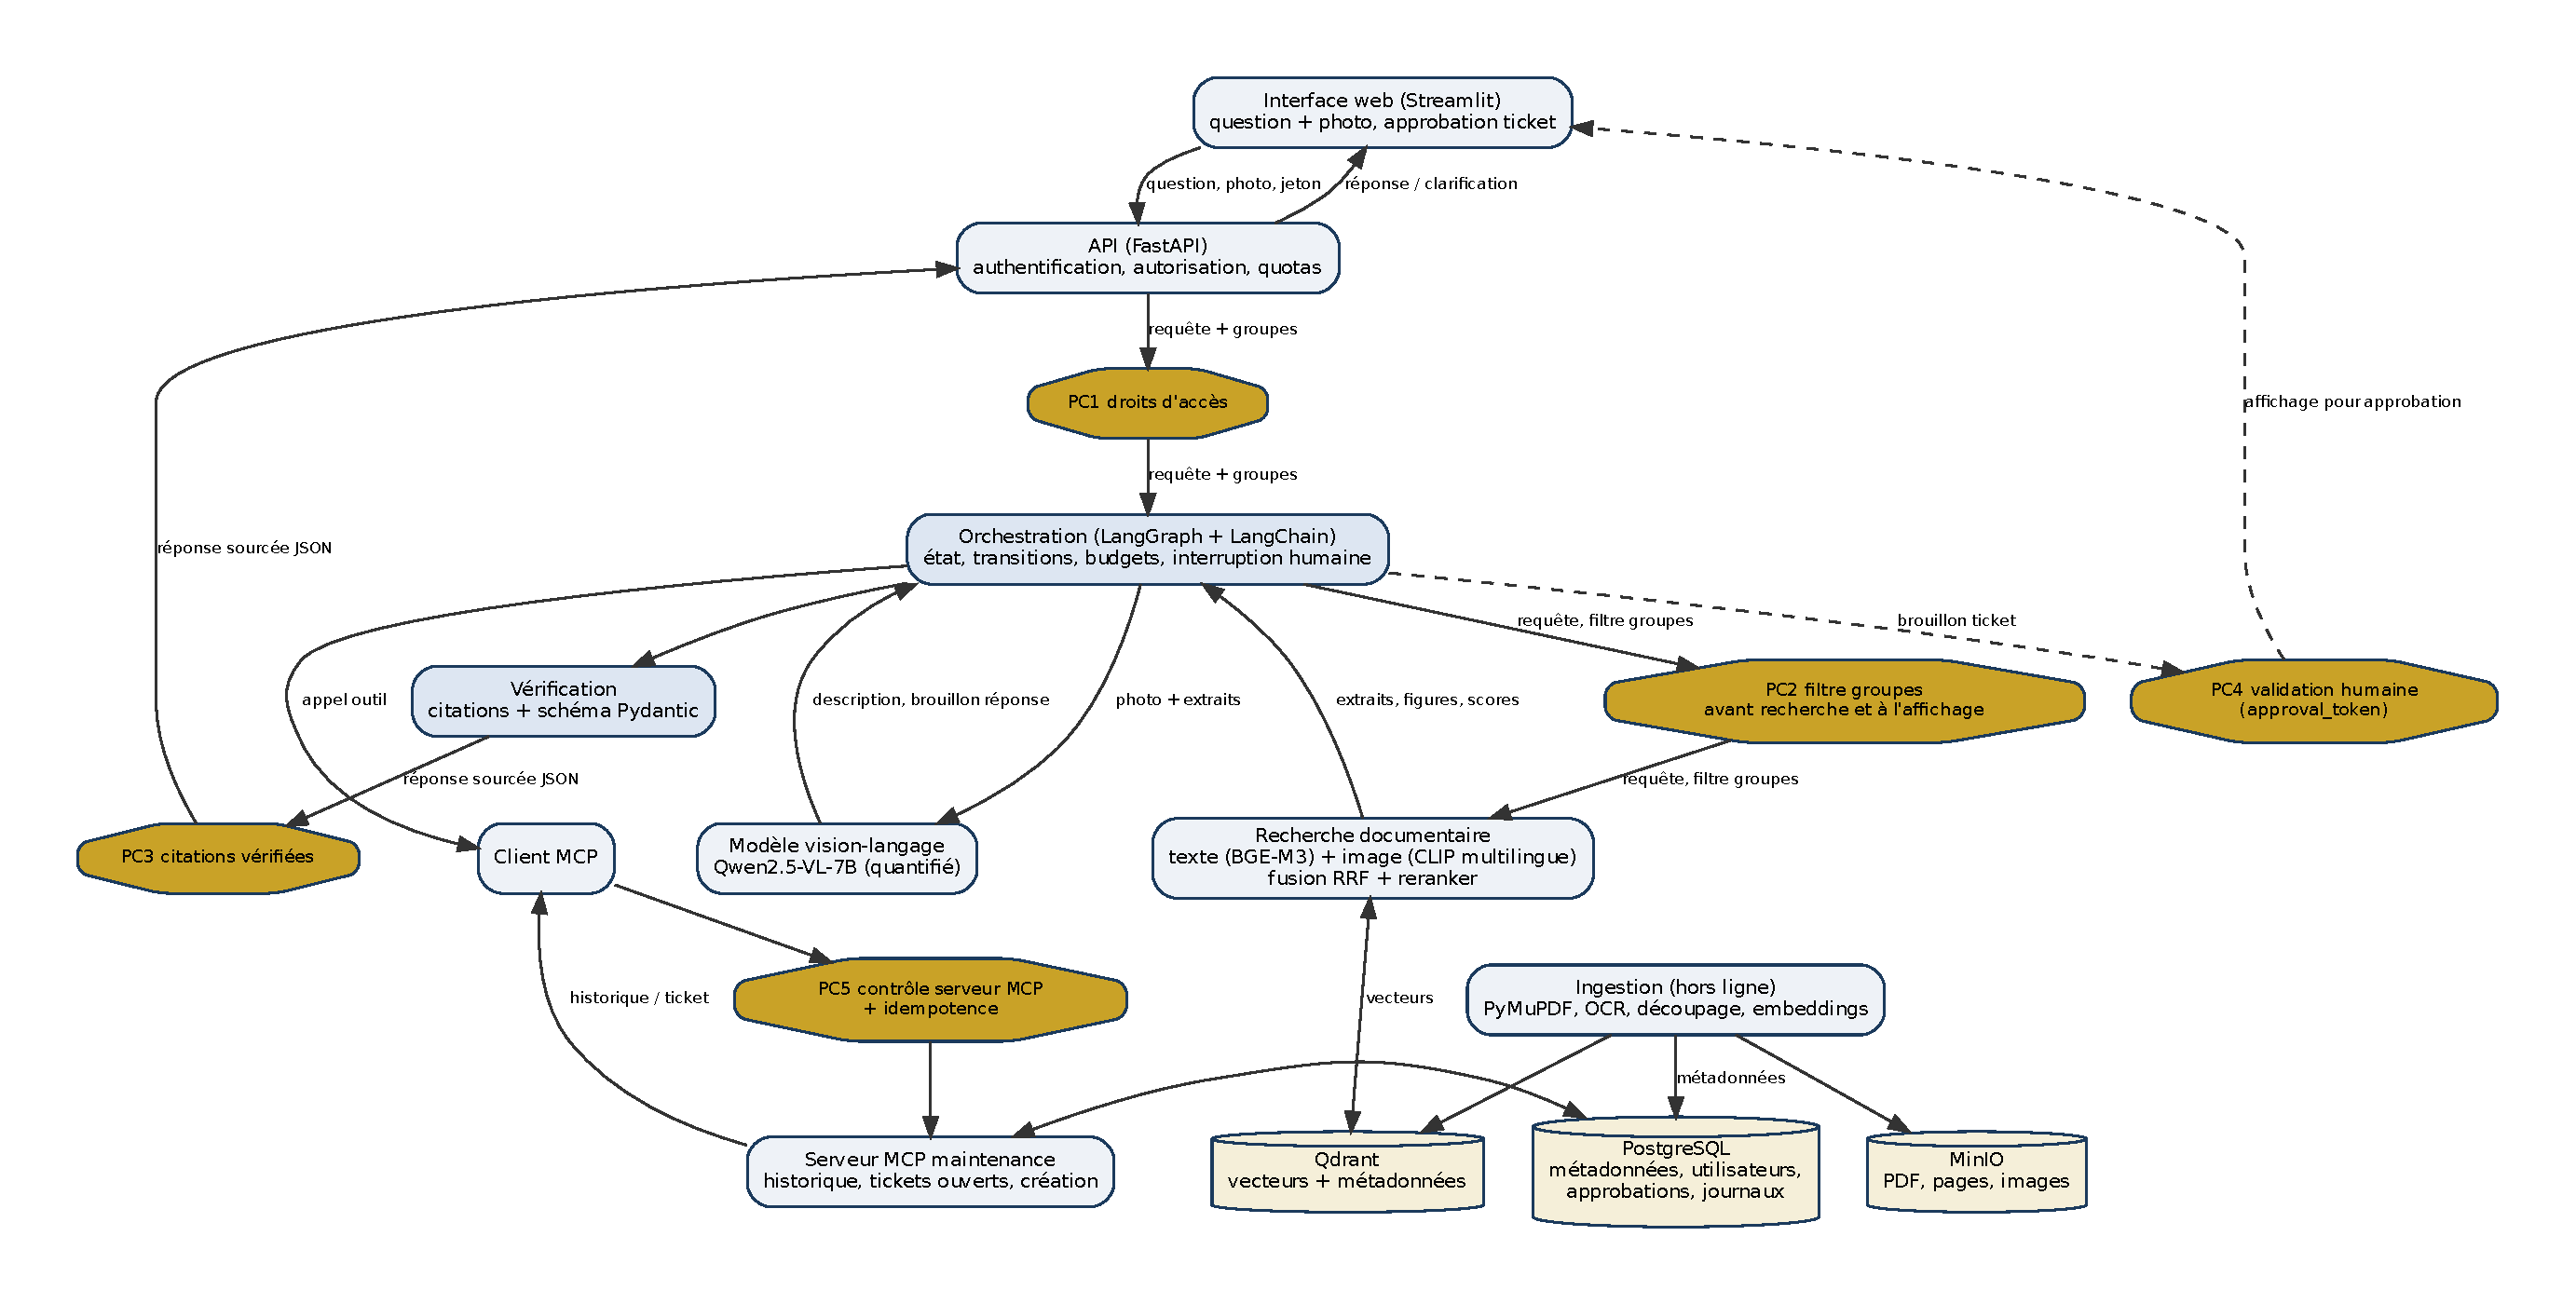
\includegraphics[width=\linewidth]{../diagrammes/architecture.pdf}
\caption{Architecture fonctionnelle de MaintiDoc. Les octogones dorés sont les points de contrôle PC1 à PC5.}
\end{figure}

\begin{center}
\begin{tabularx}{\linewidth}{lL{3.3cm}X}
\toprule
\textbf{PC} & \textbf{Où} & \textbf{Ce qui est vérifié}\\\midrule
PC1 & API, à l'entrée & identité (jeton), groupes de l'utilisateur, quotas et taille de la photo\\
PC2 & avant la recherche et à l'affichage & filtre Qdrant sur \texttt{groupes\_acces} ; nouveau contrôle avant d'ouvrir un PDF ou une image\\
PC3 & après la génération & chaque citation pointe vers un élément récupéré, autorisé, et qui soutient l'affirmation\\
PC4 & interruption LangGraph & l'utilisateur voit et approuve le contenu exact du ticket\\
PC5 & serveur MCP & droits vérifiés à chaque appel, jeton d'approbation lié au contenu, clé d'idempotence\\
\bottomrule
\end{tabularx}
\end{center}

\newpage
\subsection{Fiches des blocs}
\begin{center}\small
\begin{longtable}{L{2.3cm}L{3.9cm}L{2.9cm}L{3.0cm}L{2.8cm}}
\toprule
\textbf{Bloc} & \textbf{Rôle} & \textbf{Entrées} & \textbf{Sorties} & \textbf{Outil envisagé}\\\midrule\endhead
Interface & Saisir la question et la photo, afficher la réponse sourcée et le ticket à approuver & texte, image, clic d'approbation & requête HTTP & Streamlit\\
API & Authentifier, autoriser, appliquer quotas et budgets, journaliser & requête, jeton & état initial du workflow, réponse JSON & FastAPI + Pydantic\\
Orchestration & Enchaîner analyse, recherche, outils, vérification ; gérer l'état, les boucles et l'interruption humaine & question, photo, groupes & réponse, clarification ou brouillon de ticket & LangGraph + LangChain\\
Recherche documentaire & Trouver passages et figures pertinents parmi les seuls documents autorisés & requête, description d'image, filtre groupes & top-k éléments + métadonnées & Qdrant, BGE-M3, encodeur CLIP multilingue, RRF, reranker\\
Modèle vision-langage & Décrire la photo, identifier l'équipement, rédiger la réponse à partir des extraits & photo, extraits, figures & description, brouillon structuré & Qwen2.5-VL-7B 4 bits (Transformers), repli 3B\\
Outil MCP & Fournir l'historique et les tickets, créer un ticket approuvé & \texttt{equipment\_id}, contenu, jeton & historique, tickets, n° de ticket & SDK MCP Python (à préciser)\\
Stockage & Conserver vecteurs, métadonnées, fichiers, approbations et journaux & éléments ingérés & données persistantes & Qdrant, PostgreSQL, MinIO\\
Ingestion (hors ligne) & Découper, OCRiser, vectoriser les documents & PDF, images, inventaire & éléments indexés & PyMuPDF, OCR local (Tesseract ou PaddleOCR, à préciser)\\
Vérification & Contrôler le format et les citations & brouillon, éléments récupérés & réponse validée ou abstention & Pydantic + prompt \texttt{evidence\_check}\\
\bottomrule
\end{longtable}
\end{center}

\subsection{Parcours d'une requête}
\begin{idee}[« Voici la photo du panneau de COMP-V-01, que signifie le voyant orange ? »]
\begin{enumerate}
\item L'API reconnaît \texttt{tech\_comp\_01} (groupe \texttt{techniciens\_compresseurs}) et vérifie la taille de la photo (PC1).
\item Le VLM décrit la photo : contrôleur CV-37, voyant H2 orange, écran éteint. L'équipement est probable, mais le code n'est pas visible.
\item La recherche texte et image s'exécute uniquement sur les documents du groupe (PC2). Elle remonte la figure 5.1 et le tableau 5.1 du manuel CV-37, puis le tableau 6.1 des codes. Le manuel PC-80, visuellement proche, est exclu par le filtre.
\item Le reranker reclasse les candidats. La réponse est rédigée : « orange = alerte ou entretien dû, six codes possibles ».
\item PC3 vérifie que chaque citation (manuel\_compresseur\_v, p.5, figure 5.1 ; p.6, tableau 6.1) existe et soutient l'affirmation.
\item Comme le code est inconnu, le statut est \texttt{needs\_clarification} : « Pouvez-vous allumer l'écran et photographier le code ? ». Aucune action n'est proposée.
\end{enumerate}
\end{idee}

\subsection{Questions ouvertes et hypothèses à vérifier}
\begin{enumerate}[label=\textbf{H\arabic*}]
\item Qwen2.5-VL-7B en 4 bits tient-il sur le T4 16 Go avec 2 à 3 images et environ 6 000 tokens de contexte, en moins de 60 s ? Sinon, faut-il passer au modèle 3B ?
\item vLLM est-il utilisable sur T4 pour ce modèle, ou faut-il rester sur Transformers ?
\item Comment exposer un VLM hébergé sur Colab aux services locaux de façon sûre (tunnel authentifié) ? Ou faut-il plutôt évaluer en mode batch sur Colab ?
\item Faut-il passer tous les documents à l'OCR, ou seulement les PDF scannés et les photos ? Quelle qualité sur les valeurs numériques (cf. « 46,061 ») ?
\item Les figures doivent-elles être indexées par l'image seule (CLIP) ou aussi par une légende générée hors ligne ?
\item Quelle granularité de découpage choisir : paragraphe, tableau entier ou page ?
\item Le reranker multilingue d'origine distingue-t-il déjà A04 (PC-80, 80 °C) de B04 (PC-150, 85 °C) ? Cette mesure servira de base au fine-tuning.
\end{enumerate}
Versions exactes, licences des outils et mémoire GPU mesurée : à préciser dans le dépôt à partir de la semaine 2.

% ================================================================== 2.4
\section{Flux de données}
\subsection{Flux d'ingestion}
\begin{center}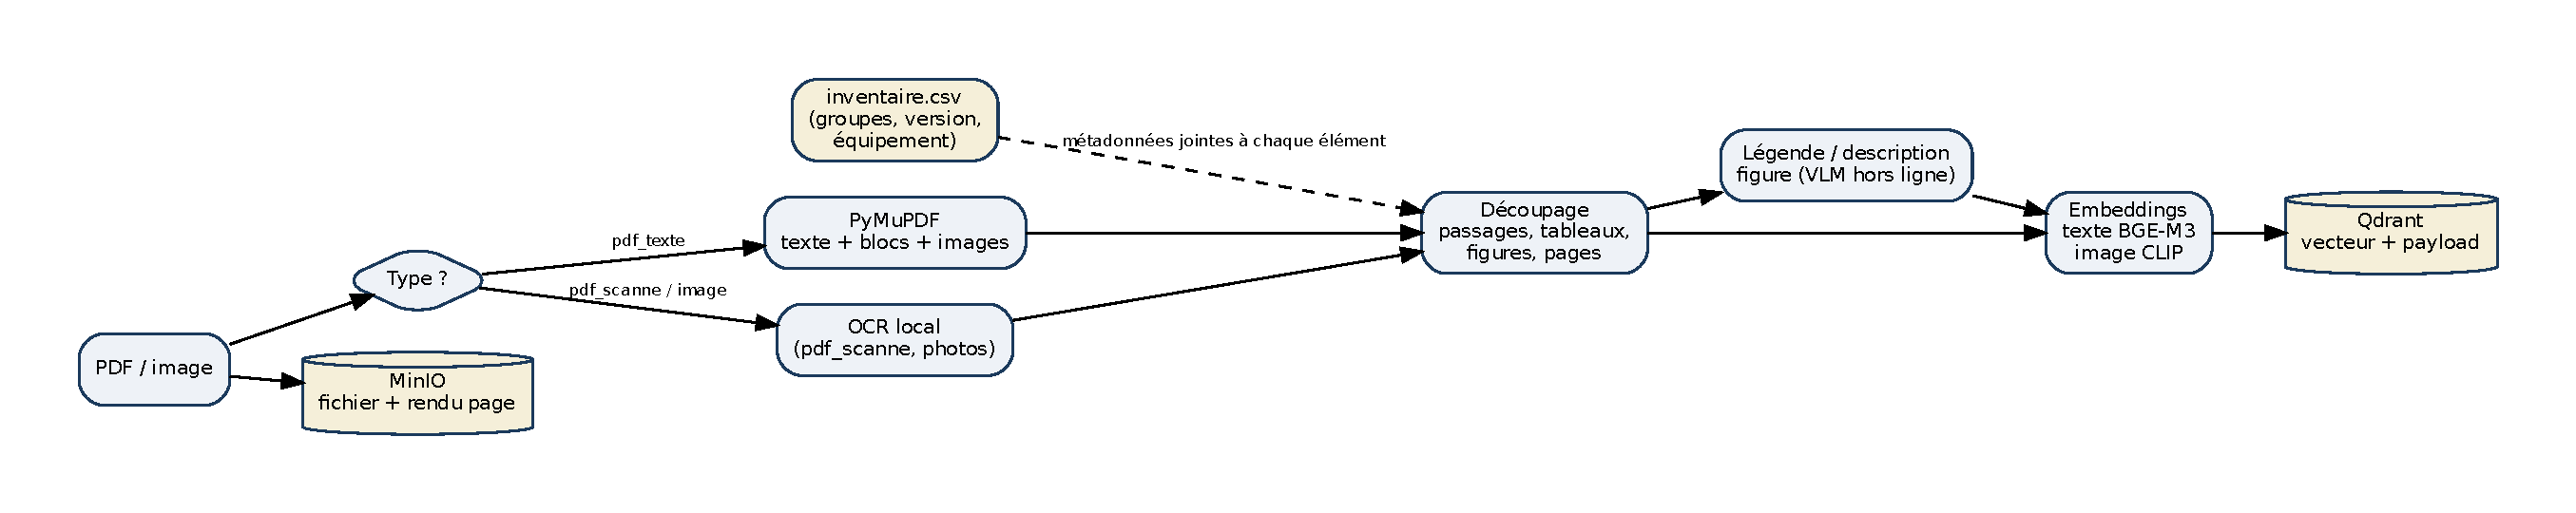
\includegraphics[width=\linewidth]{../diagrammes/flux_ingestion.pdf}\end{center}
Chaque fichier est stocké dans MinIO. Les PDF texte sont lus avec PyMuPDF (texte, blocs, images). Les PDF scannés et les photos passent par l'OCR. Le découpage produit des éléments de type passage, tableau, figure ou page, chacun avec son rendu image et ses métadonnées issues de \texttt{inventaire.csv}. Les éléments sont ensuite vectorisés : en texte avec BGE-M3, en image avec l'encodeur CLIP.

\subsection{Flux d'une requête}
\begin{minipage}[t]{0.42\linewidth}\vspace{0pt}
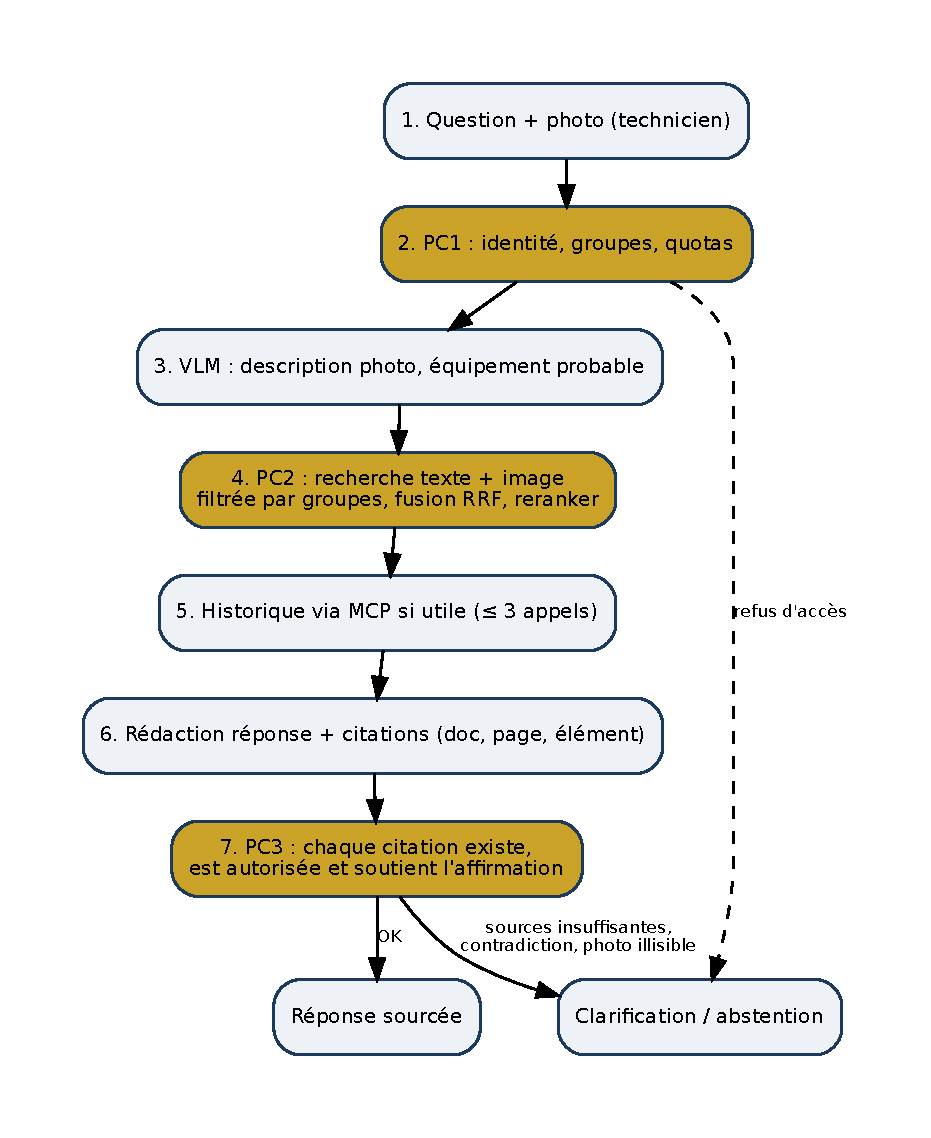
\includegraphics[width=\linewidth]{../diagrammes/flux_requete.pdf}
\end{minipage}\hfill
\begin{minipage}[t]{0.54\linewidth}\vspace{0pt}
Le contrôle d'accès intervient \textbf{trois fois} : à l'entrée (PC1), dans la requête vectorielle elle-même (PC2, filtre de payload Qdrant, donc avant tout classement) et à l'ouverture d'un document ou d'une image cités. Les extraits récupérés sont transmis au modèle dans une section balisée comme \emph{données}, jamais comme instructions.

Budgets appliqués par le code : au plus 3 appels MCP, au plus 6 appels au modèle et 60 s de traitement automatique.

L'abstention est déclenchée par l'une de ces situations : photo illisible, aucune source autorisée pertinente, documents contradictoires sans version en vigueur identifiable, ou demande dépassant le rôle documentaire (« arrête la pompe »).
\end{minipage}

\subsection{Flux de création de ticket}
\begin{center}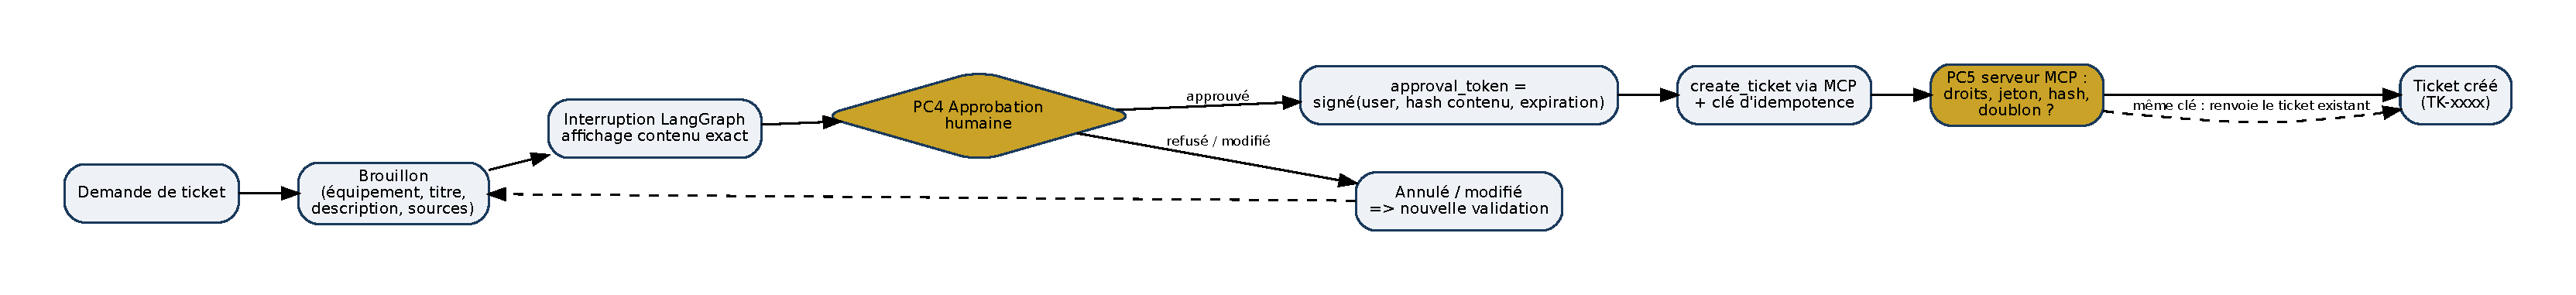
\includegraphics[width=\linewidth]{../diagrammes/flux_ticket.pdf}\end{center}
Le jeton d'approbation est signé côté serveur et lie l'utilisateur, l'empreinte SHA-256 du contenu exact (équipement, titre, description) et une date d'expiration. Toute modification du brouillon change l'empreinte et impose une nouvelle validation. La clé d'idempotence est dérivée de l'empreinte du contenu et de l'identifiant d'approbation : un second appel identique renvoie le ticket existant au lieu d'en créer un nouveau.

\subsection{Métadonnées d'un élément indexé}
\begin{center}\small
\begin{tabularx}{\linewidth}{L{4.2cm}L{4.6cm}X}
\toprule
\textbf{Champ} & \textbf{Exemple} & \textbf{Usage}\\\midrule
\texttt{element\_id} & \texttt{manuel\_pompe\_a:p6:fig6.1} & identifiant stable cité dans la réponse\\
\texttt{document\_id}, \texttt{version} & \texttt{manuel\_pompe\_a}, v3.1 (2025-03) & citation, détection des versions contradictoires\\
\texttt{page}, \texttt{type\_element} & 6, \texttt{figure} & citation de page ; passage, tableau, figure ou page\\
\texttt{famille}, \texttt{equipement\_ids}, \texttt{modele} & pompes, [POMPE-A-01, POMPE-A-02], PC-80 & filtrage et désambiguïsation\\
\texttt{groupes\_acces} & [techniciens\_pompes, responsables] & filtre PC2 (obligatoire, jamais vide)\\
\texttt{langue}, \texttt{source\_ocr} & fr, false & pondération et confiance du texte extrait\\
\texttt{usage\_test}, \texttt{statut} & normal, en\_vigueur & évaluation ; une version remplacée n'est jamais présentée comme en vigueur\\
\texttt{minio\_uri}, \texttt{bbox} & \texttt{s3://corpus/...}, [x0,y0,x1,y1] & ouverture de l'image ou de la page pour le VLM et l'affichage\\
\bottomrule
\end{tabularx}
\end{center}

\subsection{Modèle d'accès}
\begin{center}
\begin{tabularx}{\linewidth}{L{4.9cm}L{3.0cm}X}
\toprule
\textbf{Groupe} & \textbf{Utilisateurs fictifs} & \textbf{Documents accessibles}\\\midrule
\texttt{techniciens\_pompes} & tech\_pompe\_01, tech\_pompe\_02 & 22 documents : toute la famille pompes sauf le plan préventif\\
\texttt{techniciens\_compresseurs} & tech\_comp\_01 & 20 documents : la famille compresseurs sauf le plan préventif et la note de service, plus la fiche de consignation commune\\
\texttt{responsables} & resp\_maint\_01 & les 44 documents, dont 3 réservés : les 2 plans préventifs (charges et coûts) et la note de service\\
\bottomrule
\end{tabularx}
\end{center}
Règle : un utilisateur voit un élément si l'intersection entre ses groupes et \texttt{groupes\_acces} est non vide. Les tickets et l'historique MCP suivent la même règle : un technicien n'agit que sur les équipements de sa famille.

% ================================================================== 2.5
\section{Analyse des risques}
Score = probabilité $\times$ impact (de 1 à 9). En gras : les risques dont le score est supérieur ou égal à 6.
\begin{center}\small
\begin{longtable}{L{3.4cm}L{1.6cm}ccL{6.0cm}L{1.6cm}}
\toprule
\textbf{Risque} & \textbf{Catégorie} & \textbf{P} & \textbf{I} & \textbf{Mesure prévue} & \textbf{Resp.}\\\midrule\endhead
\textbf{Hallucination ou citation non fondée} & Technique & 3 & 3 & citations limitées aux éléments récupérés, contrôle PC3, abstention si sources insuffisantes, test sur 20 cas & Salah\\
\textbf{Fuite entre groupes d'accès} & Sécurité & 2 & 3 & filtre dans la requête Qdrant (pas en post-filtrage seul), contrôle à l'ouverture des fichiers, 20 tests d'accès & Adam\\
\textbf{Création de ticket non approuvée} & Sécurité & 2 & 3 & interruption LangGraph, jeton lié à l'utilisateur et au contenu, vérification par le serveur MCP & Adam\\
\textbf{Injection de prompt (document, OCR, réponse MCP)} & Sécurité & 2 & 3 & contenus balisés comme données, outils restreints, pas de réseau sortant, 2 documents piégés et 20 tests & Adam\\
\textbf{VLM trop lourd pour le T4 16 Go} & Technique & 3 & 3 & quantification 4 bits, images réduites, repli Qwen2.5-VL-3B, benchmark mémoire en semaine 3 & Salah\\
\textbf{Erreurs introduites par l'IA dans le corpus} & Données & 3 & 2 & référentiel unique, script \texttt{check.py}, relecture croisée de chaque document par l'autre membre & Salah, Adam\\
Licences des documents & Données & 1 & 3 & corpus 100 \% synthétique et marqué sur chaque page ; tout ajout public est vérifié et tracé & Adam\\
\textbf{Sessions Colab interrompues ou quota épuisé} & Organisation & 3 & 2 & sauvegarde des index et des poids sur Drive, Kaggle en secours, évaluations en lots & Salah\\
Mauvais OCR des valeurs numériques & Technique & 2 & 2 & OCR limité aux scannés, signalement \texttt{source\_ocr}, test sur les 3 scannés & Salah\\
Confusion entre équipements visuellement proches & Technique & 2 & 3 & identification obligatoire (plaque, écran), filtre par modèle, clarification si doute & Salah\\
Doublons de tickets & Technique & 2 & 2 & clé d'idempotence, \texttt{get\_open\_tickets} appelé avant le brouillon & Adam\\
Retard lié à la charge (stage, autres modules) & Organisation & 2 & 2 & planning avec marge, périmètre minimal défini (MVP en semaine 4), point hebdomadaire & Salah, Adam\\
\bottomrule
\end{longtable}
\end{center}

% ================================================================== 2.6
\section{Planning et organisation de l'équipe}\label{sec:planning}
\subsection{Répartition des rôles}
\begin{center}
\begin{tabularx}{\linewidth}{L{3cm}X}
\toprule
\textbf{Membre} & \textbf{Responsabilités principales}\\\midrule
Salah ELMECHRAFI & ingestion et OCR, recherche multimodale (Qdrant, embeddings, RRF), intégration du VLM et benchmark GPU, fine-tuning du reranker, suivi MLflow\\
Adam GHZAOUNI & API FastAPI et authentification, contrôle d'accès, serveur et client MCP, workflow LangGraph avec validation humaine, interface Streamlit, Docker Compose\\
Partagé & corpus et relecture croisée, jeu de test d'environ 150 scénarios, tests d'injection, rapports et démonstration\\
\bottomrule
\end{tabularx}
\end{center}

\newpage
\subsection{Planning des semaines 2 à 6}
\begin{center}
\begin{ganttchart}[hgrid, vgrid, x unit=2.45cm, y unit chart=0.52cm, bar height=0.55,
  bar/.append style={fill=navy!70}, group/.append style={fill=gold},
  milestone/.append style={fill=gold}, title label font=\small\bfseries, bar label font=\footnotesize]{2}{6}
\gantttitle{S2}{1}\gantttitle{S3}{1}\gantttitle{S4}{1}\gantttitle{S5}{1}\gantttitle{S6}{1}\\
\ganttbar{Ingestion, OCR, index (S)}{2}{2}\\
\ganttbar{API, accès, groupes (A)}{2}{2}\\
\ganttbar{VLM + benchmark T4 (S)}{3}{3}\\
\ganttbar{Citations, Pydantic (S, A)}{3}{3}\\
\ganttbar{Serveur MCP (A)}{3}{4}\\
\ganttbar{LangGraph + validation (A)}{4}{4}\\
\ganttbar{Paires reranker (S)}{4}{4}\\
\ganttmilestone{MVP de bout en bout}{4}\\
\ganttbar{Fine-tuning reranker (S)}{5}{5}\\
\ganttbar{Évaluation 150 scénarios (S, A)}{5}{5}\\
\ganttbar{Docker, optimisations (A)}{6}{6}\\
\ganttbar{Fiche limites, démo (S, A)}{6}{6}
\end{ganttchart}
\end{center}
Le jalon de la fin de semaine 4 est un MVP de bout en bout (question, photo, réponse sourcée, ticket approuvé). Si le VLM 7B ne tient pas sur le T4 (H1), le modèle 3B est adopté dès la semaine 3 pour ne pas bloquer la suite. Les 800 à 1 500 paires du reranker seront construites dès la semaine 4 à partir du corpus, en séparant les données par famille d'équipements.

\vspace{4pt}
\begin{idee}[Dépôt et livrables]
Le dépôt GitHub contient \texttt{corpus/} (documents, inventaire, prompts), \texttt{docs/diagrammes/} (sources Graphviz des 4 diagrammes) et \texttt{scripts/corpus/} (génération et contrôle de cohérence du corpus). Aucun secret n'y figure : un \texttt{.gitignore} exclut les fichiers \texttt{.env}, les clés et les poids de modèles.
\end{idee}

\end{document}
